% =============================================================================
% DERMA-GUARD: Evidence-Aware Specialist Consensus with Risk-Controlled
% Evidence Acquisition and Deferral for Multimodal Dermatology
%
% IEEE conference format; compiles on Overleaf with pdfLaTeX + BibTeX.
% Figures are produced by scripts/make_figures.py into paper/figures/.
% Every number comes from a script in the repository:
%   specialists, fusion rules     scripts/run_team.py      -> outputs/milk_team/team_report.json
%   decision policy, baselines    scripts/run_eade_milk.py -> outputs/eade_team/cost_*/report.json
%   statistics, fairness          scripts/analyze_milk.py  -> outputs/analysis/analysis.json
%   stress / external tests       scripts/run_stress_milk.py, run_shift_pad.py, run_shift_derm7pt.py
%   earlier prototype             scripts/legacy_pad_models.py
% =============================================================================
\documentclass[conference]{IEEEtran}
\IEEEoverridecommandlockouts

\usepackage{cite}
\usepackage{amsmath,amssymb,amsfonts}
\usepackage{graphicx}
\usepackage{textcomp}
\usepackage{xcolor}
\usepackage{booktabs}
\usepackage{multirow}
\usepackage[hidelinks]{hyperref}
\graphicspath{{figures/}}

\newcommand{\dguard}{\textsc{Derma-Guard}}
\newcommand{\HIGH}{\textsc{High}}
\newcommand{\LOW}{\textsc{Low}}
\newcommand{\ACQUIRE}{\textsc{Acquire}}
\newcommand{\DEFER}{\textsc{Defer}}
\DeclareMathOperator*{\argmax}{arg\,max}
\DeclareMathOperator*{\softmax}{softmax}

\begin{document}

\title{DERMA-GUARD: Evidence-Aware Specialist Consensus with Risk-Controlled
Evidence Acquisition and Deferral for Multimodal Dermatology}

\author{
\IEEEauthorblockN{Rachit Agarwal}
\IEEEauthorblockA{\textit{School of Computer Science and Engineering} \\
\textit{VIT Chennai}, Chennai, India \\
rachit.agarwal2022@vitstudent.ac.in}
\and
\IEEEauthorblockN{Patel Kavya Vipulkumar}
\IEEEauthorblockA{\textit{School of Computer Science and Engineering} \\
\textit{VIT Chennai}, Chennai, India \\
kavya.patel2022@vitstudent.ac.in}
\and
\IEEEauthorblockN{Aarav Prawin}
\IEEEauthorblockA{\textit{School of Computer Science and Engineering} \\
\textit{VIT Chennai}, Chennai, India \\
aarav.prawin2022@vitstudent.ac.in}
\and
\IEEEauthorblockN{Dr. Sindhu Ravindran}
\IEEEauthorblockA{\textit{School of Computer Science and Engineering} \\
\textit{VIT Chennai}, Chennai, India \\
sindhu.ravindran@vit.ac.in}
}

\maketitle

% =============================================================================
\begin{abstract}
Skin-lesion classifiers rarely fail for lack of accuracy on clean benchmarks. They fail
because they answer every case with the same apparent confidence: a blurred photograph,
missing history, or a photograph and a history that point to different diagnoses all
produce a label. We describe \dguard{}, a decision-support system that instead chooses
between four outcomes: a high-confidence answer, a request for more evidence (a
dermoscopic image, missing patient details or a better photograph), a clearly marked
low-confidence answer for a clinician to confirm, and referral when the evidence
contradicts itself. Six specialists (evidential heads for the photograph, dermoscopy and
metadata, an external legacy model, a nearest-neighbour vote and a class-balanced
embedding classifier) are profiled case by case by an evidence manager, and a learned
gate decides how much each should count; the gate was chosen from seven combination rules
under five-fold cross-fitting. A calibrated, cost-aware policy with a Learn-then-Test bound
on missed cancers makes the final choice. On 787 held-out MILK10k lesions, 89.1\% of
patients receive an answer and 57.1\% a high-confidence one that is 77.1\% accurate over
eleven diagnoses and misses 3.1\% of cancers, against 4.9\% for a learned rejector
($p=0.011$) and 3.8\% for confidence thresholding at the same coverage. Across four fusion
back-ends the policy's miss rate stays between 3.0\% and 3.5\%, while thresholding ranges
from 3.5\% to 9.3\%: abstention by confidence is only as safe as the probabilities beneath
it. Controlled image damage shows that evidential uncertainty misses blur, darkness, noise
and occlusion; explicit checks remove every confident answer on damaged input. Without
retraining, the system stays within its safety target on PAD-UFES-20 and Derm7pt, while its
fine-grained diagnosis does not transfer. Re-evaluating our earlier prototype, whose
reported accuracies of 84--90\% were not reproducible, places its models at 57--75\% on
unseen patients.
\end{abstract}

\begin{IEEEkeywords}
dermatology, multimodal fusion, evidential deep learning, selective prediction,
conformal prediction, risk control, evidence acquisition, clinical decision support
\end{IEEEkeywords}

% =============================================================================
\section{Introduction}

A patient who photographs a mole and asks an app whether it is dangerous gets an answer
almost every time. The answer comes with a number, often above 90\%, and that number
looks the same whether the photograph was sharp or blurred, whether the patient's age
and the lesion's location agree with the image, and whether the lesion resembles
anything in the training data. Deep networks reached dermatologist-level accuracy on
curated images years ago \cite{esteva2017}, so accuracy on benchmarks is no longer the
main obstacle to safe use. Behaviour is.

A careful dermatologist behaves differently. When the evidence is clear they give a
diagnosis. When it is not, they look more closely with a dermatoscope, give a provisional
opinion and ask for confirmation, or refer the patient when the history and the lesion
tell different stories. We wanted to know whether a model can be built to behave this way,
and how much it costs.

This paper is also the second attempt. The first version of \dguard{} already had the
right intuitions (a panel of specialist models, a sceptical component that questions
their evidence, and trust that depends on the suspected diagnosis), but its weights were
typed in by hand. When we audited it, its reported accuracies did not survive: the split
was made by photograph rather than by patient, and its evaluation code adjusted
predictions toward preset accuracy targets (Section~\ref{sec:legacy}). We kept the ideas,
replaced every hand-set number with one fitted on validation data, and made every result
a script that can be re-run.

\textbf{Contributions.} (i) A six-specialist team whose per-case weights are learned from
all of the evidence manager's signals, chosen from seven rules by cross-fitted validation,
with an exhaustive subset study and an oracle ceiling. (ii) A calibrated four-outcome
policy that can request three kinds of missing evidence and certifies the missed-cancer
rate of its confident answers. (iii) The finding that confidence-based abstention is only
as safe as the fusion beneath it, whereas the calibrated policy is stable across fusion
back-ends. (iv) A controlled degradation benchmark, two external tests without retraining,
and an honest re-evaluation of the earlier prototype's seven models. (v) A working care
platform, with every system variant available side by side in its interface.

% =============================================================================
\section{Related Work}

\textbf{Skin-lesion classification.} After Esteva \textit{et al.} \cite{esteva2017}, the
ISIC challenges \cite{codella2019isic} and datasets such as HAM10000
\cite{tschandl2018ham} made dermoscopic classification a standard benchmark, usually on
ImageNet-pretrained residual networks \cite{he2016resnet}; dermatology foundation models
such as PanDerm \cite{yan2025panderm} are the current frontier. Multimodal work combines
images with metadata through attention-like gating \cite{pacheco2021metablock} or uses
paired clinical and dermoscopic images \cite{kawahara2019derm7pt}. PAD-UFES-20
\cite{pacheco2020padufes} and MILK10k \cite{milk10k} provide smartphone photographs with
metadata and paired clinical--dermoscopic images, respectively, and multi-task models can
recommend when dermoscopy is needed \cite{mehta2025hotai}. None of these decide whether a
prediction should be issued at all.

\textbf{Uncertainty and evidential fusion.} Evidential deep learning \cite{sensoy2018edl}
places a Dirichlet over class probabilities and yields a per-case ignorance mass grounded
in subjective logic \cite{josang2016} and Dempster--Shafer theory
\cite{dempster1967,shafer1976}. Trusted multi-view classification \cite{han2021tmc}
combines per-view opinions with Dempster's rule so that uninformative views fall silent.
Temperature scaling \cite{guo2017calibration} and isotonic regression
\cite{zadrozny2002isotonic} calibrate confidences, and Mahalanobis distances
\cite{lee2018mahalanobis} with shrinkage covariance \cite{ledoit2004} detect unusual inputs.

\textbf{Abstention, deferral and risk control.} Chow's rule \cite{chow1970}, selective
classification \cite{geifman2017selective} and learning to defer \cite{mozannar2020defer}
decide when not to answer; AUGRC \cite{traub2024augrc} evaluates them. Conformal prediction
\cite{vovk2005,angelopoulos2021gentle,romano2020aps,sadinle2019lac}, including
class-conditional variants \cite{lu2022fair}, gives distribution-free set guarantees, and
Learn-then-Test \cite{angelopoulos2025ltt} and conformal risk control
\cite{angelopoulos2022crc} extend them to general risks. Our contribution is their
integration in one decision with learned multi-specialist evidence and measured evidence
acquisition, evaluated against simple baselines on the same probabilities.

% =============================================================================
\section{Data and Evaluation Protocol}\label{sec:data}

\textbf{MILK10k} \cite{milk10k} has 5{,}240 lesions, each with one clinical close-up and
one dermoscopic image, eleven diagnoses (95.7\% confirmed by histopathology; 71.7\%
malignant), age, sex, body site, a skin-tone class and seven automatically computed
concept scores. Without patient identifiers, we split by lesion into 3{,}667 training,
786 validation and 787 test lesions, asserting that no lesion appears twice. Validation
fits everything that is fitted after the network: fusion rules, reliabilities,
calibration, conformal quantiles, the risk threshold, the acquisition estimator and every
choice between methods. The test split was scored once.

\textbf{External data.} PAD-UFES-20 \cite{pacheco2020padufes} (2{,}298 smartphone
photographs, six classes, no dermoscopy) and Derm7pt \cite{kawahara2019derm7pt} (1{,}003
lesions with both images after mapping its diagnoses onto MILK10k classes) are used only
for testing, without retraining or recalibration.

\textbf{Metrics.} For a system that may abstain we report coverage (share of
high-confidence answers), accuracy among them and the \emph{missed-cancer rate} (share of
answered malignant lesions called benign), always comparing systems at equal coverage;
macro-F1 and balanced accuracy for the rare classes; malignant-vs-benign AUROC; AUGRC
\cite{traub2024augrc}; acquisition efficiency
$\mathrm{AE}=(G_\pi-G_{\mathrm{rand}})/(G_{\mathrm{oracle}}-G_{\mathrm{rand}})$ for the
choice of whom to send for dermoscopy; and 95\% bootstrap intervals with paired tests
(2{,}000 resamples).

% =============================================================================
\section{Method}\label{sec:method}

\begin{figure*}[t]
\centering
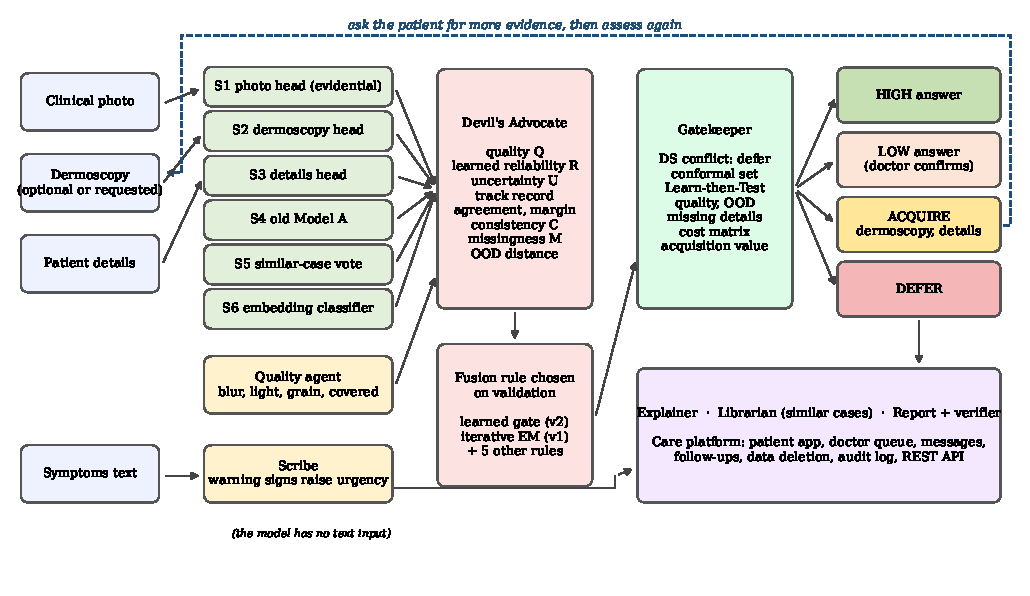
\includegraphics[width=0.94\textwidth]{fig_architecture}
\caption{\dguard{}. Six specialists are profiled by the evidence manager (``Devil's
Advocate'') and combined by the fusion rule chosen on validation; the gatekeeper and a
cost matrix choose one of four outcomes. The dashed loop is the request for more evidence,
after which the case is assessed again.}
\label{fig:arch}
\end{figure*}

Fig.~\ref{fig:arch} shows the pipeline. A case moves left to right: specialists give
opinions, the evidence manager profiles them, a fusion rule turns the profile into
weights, and the policy decides.

\subsection{Specialists}

\textbf{S1--S3: evidential heads.} An ImageNet ResNet50 \cite{he2016resnet} shared by both
image types and a residual metadata network produce three 256-dimensional embeddings, each
feeding an evidential head with non-negative evidence $e_m$ \cite{sensoy2018edl}. With
$\alpha_m=e_m+1$ and $S_m=\sum_k\alpha_{m,k}$, belief and ignorance are $b_{m,k}=e_{m,k}/S_m$
and $u_m=K/S_m$; a head contributes its pignistic distribution $p_m=b_m+u_m/K$. The heads are
also combined by Dempster's rule \cite{han2021tmc},
\begin{equation}
C=\textstyle\sum_{i\neq j}b_{1,i}b_{2,j},\quad
b_k=\frac{b_{1,k}b_{2,k}+b_{1,k}u_2+b_{2,k}u_1}{1-C},\quad u=\frac{u_1u_2}{1-C},
\end{equation}
which leaves a missing modality ($u=1$) exactly without effect and separates
contradiction ($C$) from shared ignorance ($u$). The network was trained on a Kaggle GPU
for 25 epochs with modality dropout 0.25, so that it learns to say ``I don't know'' for an
absent input.

\textbf{S4: legacy model.} The earlier prototype's image model, trained on PAD-UFES-20, is
applied unchanged; its six classes are mapped to MILK10k and mixed with 10\% uniform mass
so unsupported classes are unknown rather than impossible.

\textbf{S5, S6: case-based specialists.} S5 is a vote of the 15 most similar training
lesions in embedding space, weighted by $\exp(5\,\mathrm{sim})$ \cite{cover1967knn}. S6 is a
multinomial logistic regression over all training embeddings with class weights inversely
proportional to frequency, so that rare diagnoses are not drowned out; its regularisation
was chosen on validation.

\subsection{The evidence manager}

For specialist $m$ on case $x$ the evidence manager computes ten signals: quality $Q_m$
(share of image statistics inside the training 5th--95th percentiles), a reliability
$R_m$ (logistic regression fitted on validation predicting whether $m$ is right),
normalised entropy $U_m$, confidence, margin, agreement with the other specialists, the
measured track record $\pi_m(\hat y_0)=\Pr(m\text{ correct}\mid y=\hat y_0)$ at the
provisional diagnosis, the team's Jensen--Shannon consistency \cite{lin1991js},
missingness, and the Mahalanobis out-of-distribution distance
\cite{lee2018mahalanobis,ledoit2004}. The earlier prototype multiplied hand-set versions,
$E_m=Q_mR_mU_mCSM_m$, and normalised them into weights; because consistency $C$ and
sufficiency $S$ are equal for all specialists of a case, they cancelled, and only three
signals ever moved the weights.

\subsection{Fusion rules and how one is chosen}\label{sec:fusion}

\textbf{Iterative diagnosis-adaptive fusion (v1)} keeps the prototype's EM-style loop
\cite{dempster1977em}: weights $w_m\propto(Q_mR_m)^a$ give a provisional diagnosis
$\hat y$; then up to three times
$w_m=\softmax_m\big(a\log Q_mR_m+b\log\pi_m(\hat y)+g\log\kappa_m\big)$, with
$\kappa_m=\rho$ for specialists disagreeing with $\hat y$, and the diagnosis is updated.

\textbf{The learned gate (v2)} lets every signal act. With the standardised signal vector
$\phi_m(x)$,
\begin{equation}
w_m(x)=\softmax_{m\in\text{present}}\big(\beta_m+\theta_m^{\top}\phi_m(x)\big),
\end{equation}
and the opinions are pooled either as a mixture $\sum_m w_mp_m$ or as a product of experts
$\propto\prod_m p_m^{w_m}$, followed by temperature scaling. $\theta,\beta$ and the
temperature minimise validation log-loss with an $\ell_2$ penalty.

\textbf{Seven rules} are compared: simple average, the original formula with learned
reliability, the single specialist with the highest $R_m$, the iterative fusion,
stacking, and the gate with both poolings. Validation lesions serve twice (to fit fusion
and to calibrate the policy), so every rule is \emph{cross-fitted}: fitted on four fifths
of validation and applied to the remaining fifth, five times. The out-of-fold
probabilities are used both to select the rule (best macro-F1, fixed before any test
result was seen) and to calibrate the policy. We also refit the selected rule on all 31
(stage A) and 63 (stage B) specialist subsets, and report an oracle that picks, per case,
the specialist giving the true class most mass.

\subsection{The decision policy}

Stage A uses the photograph and metadata; stage B adds dermoscopy. The stated diagnosis
is the most probable class; costs are $0$ for a correct answer, $1$ within the benign or
malignant group, $c_{\mathrm{miss}}=5$ for a cancer called benign and $2$ for the reverse,
with $0.5$ to acquire dermoscopy and $1.5$ for a clinician review. Gates are: Dempster--Shafer
conflict above its validation 90th percentile (\DEFER); a Mondrian least-ambiguous
conformal set over \{benign, malignant\} ($\alpha=0.1$) \cite{sadinle2019lac,lu2022fair}
that still contains ``malignant'' when the answer would be benign; a Learn-then-Test
threshold \cite{angelopoulos2025ltt} on $1-u$ such that
$\Pr(\text{missed-cancer rate}\le0.05)\ge0.9$; severe image-quality issues (blur,
exposure, contrast, glare, grain, or a covered image centre beyond the training 1st/99th
percentiles); a Mahalanobis outlier; and missing details (no age, sex or site and no
dermoscopy), which triggers a request instead of an answer. If no gate fires and answering
is cheapest, the answer is \HIGH. Otherwise the system requests dermoscopy when the
expected cost after acquisition, estimated by a gradient-boosted regressor fitted on
validation lesions whose dermoscopy is known, plus $0.5$, is below the cost of review;
else it gives a \LOW\ answer for a clinician to confirm. Only contradiction or absent
evidence leads to \DEFER, so the \HIGH\ tier coincides with a conventional
defer-on-any-gate policy and all baseline comparisons concern the same answers.

\subsection{Agents and platform}

Around the policy, a quality agent advises on retakes, a scribe raises triage urgency when
the patient's own words mention warning signs (with negation handling; it never changes
the diagnosis), a librarian shows similar confirmed \emph{training} lesions
\cite{lewis2020rag}, an explainer states who said what, why dissenting specialists
disagree and where the weight went, and a report writer may use a local language model
whose output is discarded if a verifier finds any diagnosis or percentage not in the
evidence. A care platform routes each outcome to the patient or a clinician queue, keeps
an audit log and lets patients delete their data. Its interface runs any lesion through
every specialist, fusion rule and baseline side by side.

% =============================================================================
\section{Results}\label{sec:results}

\subsection{Specialists and fusion}

\begin{table}[t]
\centering
\caption{Specialists alone and the main fusion rules on the test split (stage B: with
dermoscopy). Val: out-of-fold validation macro-F1 used for selection.}
\label{tab:fusion}
\setlength{\tabcolsep}{3pt}
\small
\begin{tabular}{lccccc}
\toprule
 & Val & Acc. & F1 & Bal. & AUROC \\
\midrule
\multicolumn{6}{l}{\emph{Specialists (stage B)}} \\
S1 photograph head & -- & 0.595 & 0.264 & 0.266 & 0.787 \\
S2 dermoscopy head & -- & 0.705 & 0.400 & 0.411 & 0.854 \\
S3 metadata head & -- & 0.600 & 0.246 & 0.252 & 0.749 \\
S4 legacy model & -- & 0.219 & 0.077 & 0.096 & 0.553 \\
S5 nearest-neighbour vote & -- & 0.719 & 0.431 & 0.402 & 0.866 \\
S6 embedding classifier & -- & 0.700 & 0.440 & \textbf{0.447} & 0.875 \\
\midrule
\multicolumn{6}{l}{\emph{Fusion, stage A (photograph + metadata)}} \\
Dempster--Shafer, heads & 0.274 & 0.644 & 0.286 & 0.280 & 0.799 \\
Simple average & 0.344 & 0.637 & 0.343 & 0.338 & 0.824 \\
Iterative EM (v1) & 0.374 & 0.670 & \textbf{0.383} & \textbf{0.375} & 0.832 \\
Stacking & 0.272 & 0.644 & 0.308 & 0.296 & 0.822 \\
Learned gate (v2)$^\star$ & \textbf{0.412} & 0.657 & 0.377 & 0.360 & \textbf{0.838} \\
\midrule
\multicolumn{6}{l}{\emph{Fusion, stage B (+ dermoscopy)}} \\
Dempster--Shafer, heads & 0.361 & 0.690 & 0.376 & 0.378 & 0.856 \\
Simple average & 0.457 & 0.714 & 0.422 & 0.400 & 0.870 \\
Iterative EM (v1) & 0.492 & 0.717 & \textbf{0.459} & \textbf{0.444} & 0.862 \\
Stacking & 0.413 & 0.720 & 0.372 & 0.361 & 0.853 \\
Learned gate (v2)$^\star$ & \textbf{0.517} & \textbf{0.731} & 0.438 & 0.418 & \textbf{0.885} \\
\emph{Oracle best specialist} & -- & 0.840 & 0.594 & -- & -- \\
\bottomrule
\multicolumn{6}{l}{\footnotesize $^\star$selected (product pooling). All seven rules: Fig.~\ref{fig:fusion}.}
\end{tabular}
\end{table}

\begin{figure*}[t]
\centering
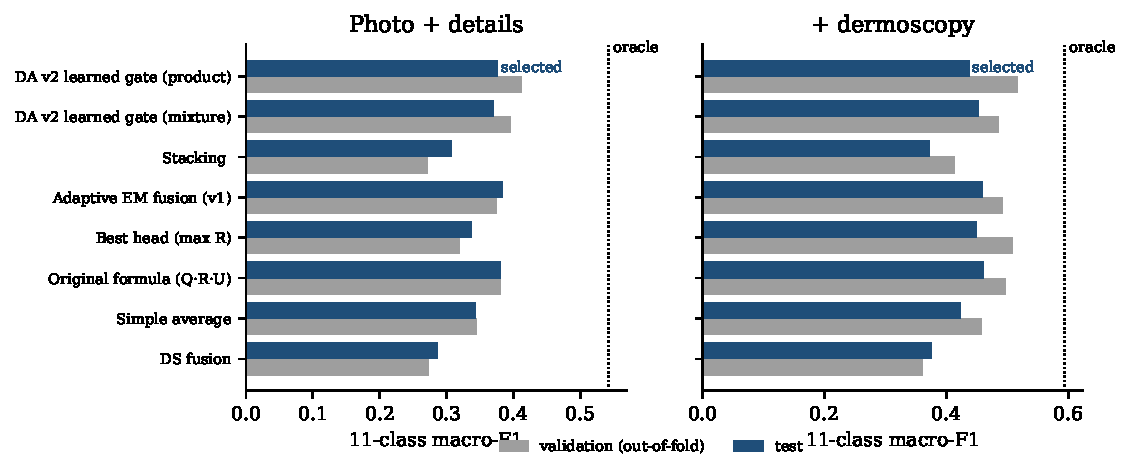
\includegraphics[width=0.86\textwidth]{fig_fusion_rules}
\caption{All seven combination rules: out-of-fold validation macro-F1 (grey, used to
select) and test macro-F1 (blue). The dotted line is the oracle that always picks the
best specialist.}
\label{fig:fusion}
\end{figure*}

Table~\ref{tab:fusion} and Fig.~\ref{fig:fusion} summarise the specialists and the fusion
rules. Dermoscopy carries real information: the dermoscopy head beats the photograph head
on every metric, and adding it lowers the network's mean ignorance from 0.676 to 0.439. The
legacy model transfers poorly (21.9\% accuracy). The two case-based specialists are the
strongest single sources, and the class-balanced classifier S6 has the best balanced
accuracy.

Every way of weighting the team that uses the evidence beats the evidential network alone:
without dermoscopy, macro-F1 rises from 0.286 to 0.377 for the selected gate, and with
dermoscopy the gate has the best accuracy (0.731) and AUROC (0.885). The gate won the
cross-fitted validation comparison in both stages; on test the iterative fusion has a
slightly higher macro-F1, a reminder that macro-F1 over classes with fewer than ten test
lesions is noisy. We kept the pre-declared choice. Stacking, the textbook learned
combiner, is the weakest learned rule: 66 free inputs and 786 validation lesions are not
enough. Adding S6 raised the selected rule's stage-A macro-F1 from 0.332 to 0.377, and the
subset study found no subset that beat the full team by more than 0.033 on validation.
The oracle's 0.594 shows that per-case \emph{selection}, not the specialists, is the
bottleneck. On average the gate gives the largest weights to the metadata head (0.35--0.41)
and S6 (0.21--0.22), moves weight to dermoscopy when it is present, and gives the legacy
model 0.07. Isotonic calibration makes the displayed confidence honest: 0.757 shown on
average against 0.731 actual accuracy with dermoscopy, 0.660 against 0.657 without.

\subsection{Decisions}

\begin{table}[t]
\centering
\caption{Decision policy and baselines on the same probabilities (test, $c_{\mathrm{miss}}=5$).
Abstaining baselines are matched to \dguard{}'s coverage.}
\label{tab:policy}
\setlength{\tabcolsep}{2.8pt}
\small
\begin{tabular}{lccccc}
\toprule
Policy & Ans. & Derm. & Acc. & Missed & Cost \\
\midrule
Always answer, photograph & 100\% & 0\% & 0.657 & 7.2\% & \textbf{0.759} \\
Always acquire, answer & 100\% & 100\% & 0.731 & 6.4\% & 1.124 \\
Confidence threshold (B3) & 57.1\% & 0\% & \textbf{0.815} & 3.8\% & 0.881 \\
Learned rejector (L2D) & 57.1\% & 0\% & 0.764 & 4.9\% & -- \\
Entropy-chosen acquisition & 100\% & 29.5\% & 0.700 & 5.6\% & 0.790 \\
\textbf{\dguard{}, \HIGH\ tier} & 57.1\% & 29.5\% & 0.771 & \textbf{3.1\%} & 1.047 \\
\midrule
\multicolumn{6}{l}{\dguard{} outcomes: \HIGH\ 57.1\%, \LOW\ 32.0\% (top-3 85.7\%), \DEFER\ 10.9\%}\\
\bottomrule
\end{tabular}
\end{table}

\dguard{} answers 89.1\% of patients (Table~\ref{tab:policy}). Its 57.1\% high-confidence
answers are 77.1\% accurate (95\% CI 73.0--80.8\%) and miss 3.1\% of the cancers they
answer (1.6--4.8\%); Learn-then-Test certified thresholds at both stages
($\hat\lambda=0.218$, $0.276$). Low-confidence answers are right only 49.6\% of the time,
which is why they always go to a clinician, but the truth is in their top three for 85.7\%.
Dermoscopy was requested for 29.5\% of patients.

At the same coverage, a learned rejector trained to predict the model's own errors
\cite{mozannar2020defer} misses 4.9\% of cancers, significantly more than \dguard{}
($+1.8$ points, CI $+0.2$ to $+3.5$, one-sided $p=0.011$). Plain confidence thresholding
misses 3.8\%; the difference ($+0.7$ points, CI $-0.7$ to $+2.0$, $p=0.18$) is not
significant, and thresholding is more accurate (81.5\% vs.\ 77.1\%) because it answers only
the photograph's easiest cases. Always answering is cheapest in mean cost, since every
clinician review is charged 1.5.

\begin{figure}[t]
\centering
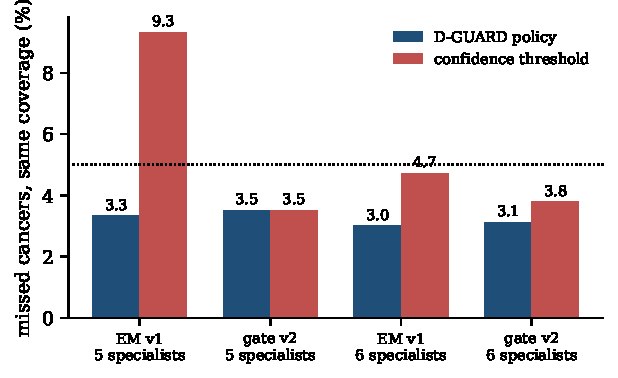
\includegraphics[width=\columnwidth]{fig_backend_robustness}
\caption{The identical policy over four fusion back-ends (iterative EM or learned gate,
with five or six specialists). The policy's missed-cancer rate stays at 3.0--3.5\%;
confidence thresholding at the same coverage ranges from 3.5\% to 9.3\%.}
\label{fig:backend}
\end{figure}

\textbf{Is the gap to thresholding real?} We ran the identical policy on four fusion
back-ends (Fig.~\ref{fig:backend}). Its miss rate barely moved, 3.0--3.5\%. The
threshold's moved almost threefold, from 3.5\% (the five-specialist gate) to 9.3\% (the
five-specialist iterative fusion). A confidence threshold is exactly as safe as the
ranking it receives, and nobody deploying it knows in advance which kind of ranking they
have; the calibrated policy delivers the same certified rate on all four. The same comparison
contains a result against us: the learned acquisition estimator chose whom to send for
dermoscopy far better than entropy on the iterative fusion (AE $+0.30$ vs.\ $-0.04$) but
worse on the final gate ($+0.07$ vs.\ $+0.26$), and ignorance ranked errors better than
softmax on the former (AUGRC 0.0874 vs.\ 0.0918) but not the latter (0.0820 vs.\ 0.0757).
Once the fused probabilities are good, simple uncertainty is a good enough guide.

Raising $c_{\mathrm{miss}}$ from 2 to 10 lowers the \HIGH\ share from 61.6\% to 53.4\% and
the miss rate from 4.1\% to 1.9\% (thresholding: 3.8\% at the same coverage), while about
89\% of patients still get an answer. Fairness is a weakness: for the 67 test lesions of
skin tone~2 the \HIGH\ miss rate is 11.5\%, against 2.2\% for tone~3 ($n=489$); tone~1 has
only 14 lesions.

\subsection{Robustness: DERMA-STRESS}

\begin{figure*}[t]
\centering
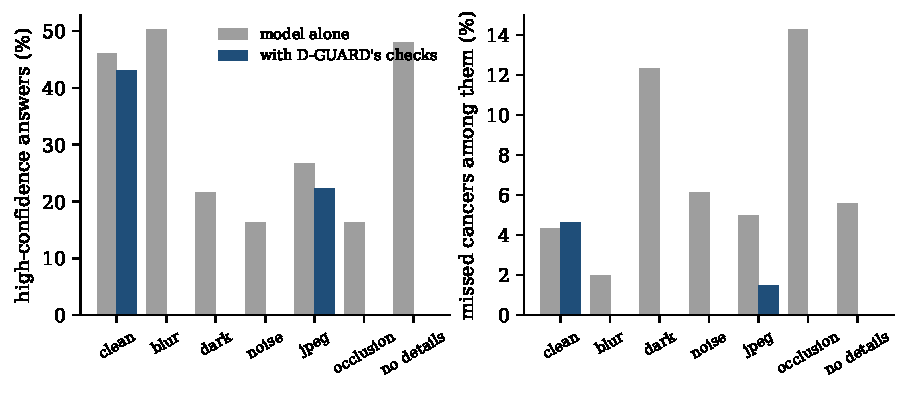
\includegraphics[width=0.82\textwidth]{fig_stress}
\caption{DERMA-STRESS on 300 test lesions (photograph + metadata): share of
high-confidence answers and missed cancers among them, for the model alone (grey) and
with the pipeline's quality and missing-details checks (blue).}
\label{fig:stress}
\end{figure*}

We damaged the photograph of 300 test lesions six ways without retraining
(Fig.~\ref{fig:stress}). Evidential ignorance does not catch what matters. Gaussian blur
\emph{lowers} mean ignorance (0.679 to 0.605) and \emph{raises} the high-confidence rate
(46\% to 50\%); under-exposed and occluded photographs keep 22\% and 16\% high-confidence
answers that miss 12.3\% and 14.3\% of cancers. Explicit checks do catch it: the quality
agent flags every blurred, dark, noisy and occluded photograph (the last two through the
grain and covered-centre checks), and every case without metadata becomes a request for
it. With these checks no damaged input received a high-confidence answer; JPEG artefacts
kept 22\% at 1.5\% missed. The price is that 8\% of clean photographs are also flagged.

\subsection{External tests}

\begin{table}[t]
\centering
\caption{The MILK10k system on two other datasets, unchanged. Threshold: confidence
thresholding at the same coverage.}
\label{tab:shift}
\setlength{\tabcolsep}{3pt}
\small
\begin{tabular}{lccc}
\toprule
 & MILK10k & PAD-UFES-20 & Derm7pt \\
\midrule
Dermoscopy available & yes & no & on request \\
Malignant share & 72\% & 79\% & 29\% \\
Photos failing quality check & 8\% & 28\% & 29\% \\
Dermoscopy requested & 30\% & 28\% & 39\% \\
Accuracy, all cases & 0.731 & 0.367 & 0.479 \\
Malignant AUROC & 0.885 & 0.840 & 0.738 \\
\HIGH\ share & 57.1\% & 11.4\% & 13.0\% \\
Accuracy of \HIGH\ answers & 0.771 & 0.517 & 0.708 \\
Missed cancers, \HIGH & 3.1\% & 0.0\% & 3.8\% \\
Threshold: missed / accuracy & 3.8\% / 0.815 & 0.0\% / 0.574 & 5.4\% / 0.846 \\
\bottomrule
\end{tabular}
\end{table}

The calibration guarantees assume that future patients resemble calibration patients.
Table~\ref{tab:shift} shows what happens when they do not. On both external datasets
ignorance, quality flags and deferrals rise and the high-confidence share falls from 57\%
to 11--13\%. Among the confident answers that remain the safety target holds: no cancer
was missed on PAD-UFES-20 and 3.8\% on Derm7pt, below thresholding's 5.4\%. On Derm7pt,
where dermoscopy exists, the system asked for it for 39\% of lesions and overall accuracy
rose from 0.402 with photographs alone to 0.479. The eleven-class diagnosis does not
transfer: half of PAD-UFES-20's confident answers are wrong, melanoma recall on Derm7pt is
31\%, and thresholding is more accurate on both datasets.

\subsection{The earlier prototype, re-evaluated}\label{sec:legacy}

\begin{figure}[t]
\centering
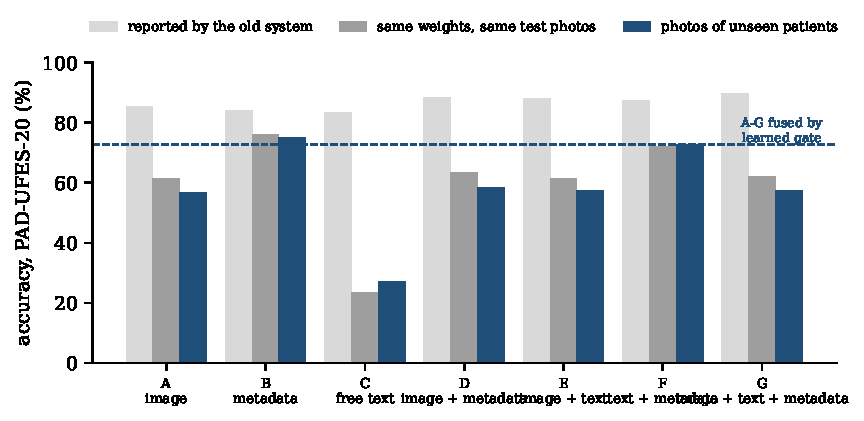
\includegraphics[width=\columnwidth]{fig_legacy_models}
\caption{The earlier prototype's seven PAD-UFES-20 models: accuracy as reported, re-scored
with the same weights on the same test photographs, and on photographs of patients never
seen in training. Dashed: the seven fused by \dguard{}'s learned gate (cross-validated).}
\label{fig:legacy}
\end{figure}

The prototype trained seven PAD-UFES-20 models (image, metadata, free text and their
combinations) and reported 84--90\% accuracy. Its split was random by photograph, so 43\%
of test photographs came from a lesion and 62\% from a patient already in training, and
its evaluation function swapped probabilities between the true class and its closest rival
until the number of correct predictions met a hard-coded target per model. Loading the
saved weights and cached features unchanged and scoring them honestly
(Fig.~\ref{fig:legacy}): on the 132 test photographs of unseen patients, the image model
reaches 56.8\%, the metadata model 75.0\%, the text model (whose ``narratives'' were
generated from the metadata) 27.3\%, and the three-modality model 57.6\%, worse than
metadata alone. Fusing the seven with our learned gate, cross-validated on those 132
photographs, gives 72.7\% against 59.8\% for averaging them; the gate recovers almost all of
the best model's accuracy without being told which model that is.

Finally, the PAD-UFES-20 questionnaire lets us test the scribe's triage rule: of 1{,}641
lesions, those with any of its warning signs were malignant (BCC, SCC or melanoma) in
48.7\% of cases against 12.4\% without (relative risk 3.9, 95\% CI 2.8--5.5), and every
single sign had a relative risk between 1.65 and 3.0.

% =============================================================================
\section{Discussion}

\textbf{What the earlier design got right.} Consulting several specialists, questioning
their evidence, and trusting them according to the suspected diagnosis all survived honest
evaluation; every evidence-aware rule beat both the evidential network alone and plain
averaging, and the measured trust table confirms clinical intuition (dermoscopy is reliable
for squamous lesions, the photograph for melanoma). What it got wrong was its evidence.

\textbf{What did not work.} Stating the minimum-cost diagnosis (classic Chow
\cite{chow1970}) labelled 98.5\% of lesions malignant on this 72\%-malignant population;
adaptive prediction sets for the safety gate collapsed to the full set and deferred every
patient; post-hoc logit adjustment raised validation macro-F1 from 0.36 to 0.44 but lowered
test macro-F1 from 0.376 to 0.359; fitting the fusion in-sample on the calibration lesions
inflated the high-confidence share by three points before cross-fitting; and classes with
fewer than ten test lesions are almost never predicted.

\textbf{Lessons about evaluation.} Split by the unit you will meet in practice; never
post-process predictions with the label; choose on validation and keep the choice when
the test disagrees; and compare against simple baselines on the same probabilities, and on
more than one model. The most useful finding of this work, that thresholding's safety is
borrowed from the fusion beneath it, appears only under that last rule.

\textbf{Limitations.} All results come from one training seed of an ImageNet ResNet50;
786 validation lesions do a great deal of fitting; MILK10k is a referral population
without patient or centre identifiers; the costs are declared, not derived; the guarantees
assume exchangeability; the image checks are heuristics; lighter skin tones are under-served;
and the system has not been evaluated in a clinic.

% =============================================================================
\section{Conclusion}

\dguard{} turns a team of imperfect specialists into calibrated clinical actions: it answers
nine in ten patients, more than half with a confident answer that misses about one cancer
in thirty, asks for dermoscopy, details or a better photograph when they are needed, and
refers only when the evidence contradicts itself. Learning how much to trust each specialist
from all of its evidence improves photograph-only diagnosis by a third. The calibrated
policy is safer than a learned rejector and, unlike confidence thresholding, stays safe
whichever fusion it is given. We hope the most transferable lesson is methodological:
report the simple baseline on the same probabilities, on more than one model, and keep
every number reproducible.

\section*{Reproducibility}
Code, per-case predictions and the script behind every table and figure are in the project
repository. Model weights and images are not redistributed; MILK10k is available from the
ISIC Archive under CC-BY-NC.

\bibliographystyle{IEEEtran}
\bibliography{refs}

\end{document}
